\section{NetFPGA Prototype}

Figure \ref{fig:proto_arch}, shows how we integrated our programmable traffic manager into the P4-NetFPGA switch architecture~\cite{P4-NetFPGA} so that we could evaluate the design on real hardware. Table \ref{tab:params} shows the design parameters that we used for the prototype. In addition to our traffic manager, we integrated modules to facilitate performance characterization. The ``Trim \& Stats'' module is designed to trim all packets to 64B and insert a 64-bit timestamp (with 5ns resolution) along with the size of the queues in the traffic manager. The rate limiter module limits the egress link bandwidth to emulate congestion.

In the subsequent sections, we provide the first demonstrations of using a programmable traffic manager to implement various common scheduling algorithms. In these demonstrations, unless otherwise noted, the 10G ingress link bandwidth is shared equally among four flows. The traffic is generated using a MoonGen~\cite{moongen} application. The P4 classifier directs each flow into a separate queue. The rate limiter is configured to limit the egress link bandwidth to 4.5 Gb/s. The only difference amongst the demonstrations described below is in the implementation of the rank computation and queue classification. These demonstrations indicate that our system is capable of running at line rate on real hardware and that the PIFO is flexible enough to be used as a primitive to implement different scheduling algorithms.


\begin{figure}[!ht]
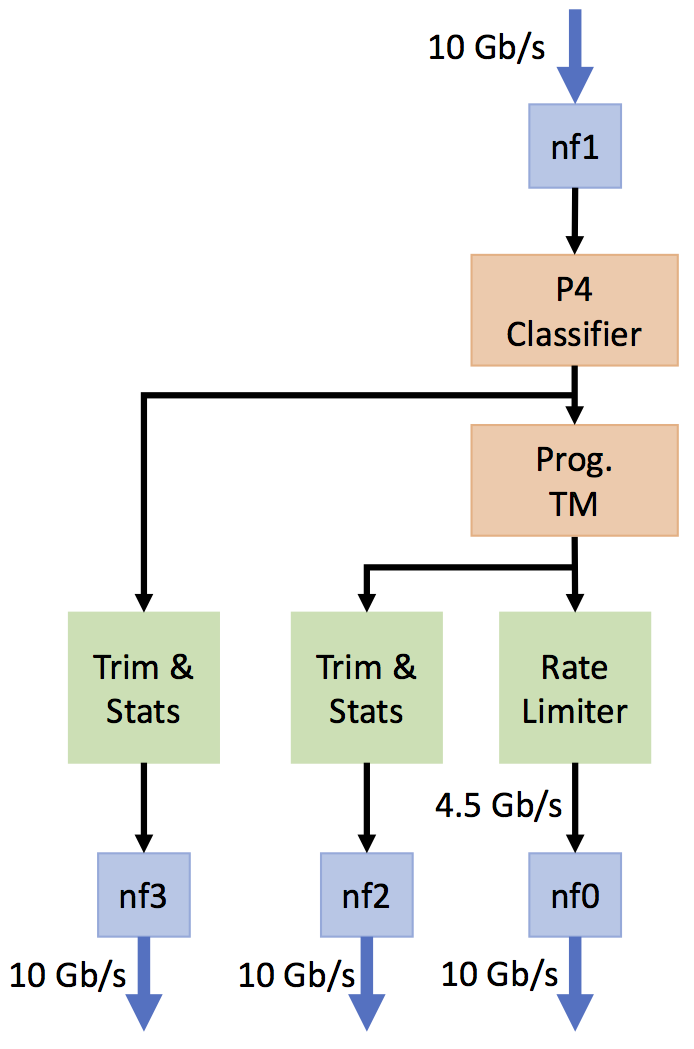
\includegraphics[width=0.7\linewidth]{figures/design/prototype_arch}
\caption{The NetFPGA pipeline used to evaluate our prototype.}
\label{fig:proto_arch}
\end{figure}

\begin{table}[tbp]
\centering
\caption{Traffic Manager Parameters Used for NetFPGA Prototype}
\label{tab:params}
\begin{tabular}{|l|l|}
\hline
\multicolumn{1}{|c|}{\textbf{Parameter}} & \multicolumn{1}{c|}{\textbf{Value}} \\ \hline
PIFO size (pkts)                         & 2048                                \\ \hline
Register Cache Size (pkts)               & 16                                  \\ \hline
Buffer size (64B segments)               & 2048                                \\ \hline
Num Skip Lists                           & 12                                  \\ \hline
Num Queues                               & 4                                   \\ \hline
\end{tabular}
\end{table}

\subsection{Strict Priority}\label{sec:strict-demo}
%\todo[inline]{Show queues sizes with 4 flows. Remove rate plots.}
The strict priority scheduling algorithm guarantees that the highest priority queue receives the full egress bandwidth so long as it has any packets in it. This algorithm would be used in scenarios with a limited amount of high priority traffic. In order to implement strict priorities with a PIFO, the rank of each packet is simply equal to its assigned queue ID, where queue 0 is the highest priority queue, then queues 1, 2, and 3, respectively.

Figure \ref{fig:strict_queues} shows the queue sizes during an experiment where four flow equally share the 10Gb/s ingress link bandwidth. After a brief startup period, the MoonGen application begins sending traffic at line rate at time 2.4 ms. As expected, since queue 0 receives the highest priority, it is mostly empty, apart for one or two packets resulting from a burst of arrivals; and queue 1 is only served whenever queue zero is empty. Similarly, queue 2 is only served when queue 1 is empty and so forth.

%Figure \ref{fig:strict_rates} shows the measured input and output flow rates to and from the traffic manager for this experiment. We see that since flow 0 is strictly prioritized and its ingress rate (2.5 Gb/s) is less than the egress link bandwidth (4.5 Gb/s) it is able to pass through the traffic manager completely unaffected. Flow 1 receives the remaining 2 Gb/s on the egress link and packets from the remaining two flows are all dropped once their queues saturate.

\begin{figure}[!ht]
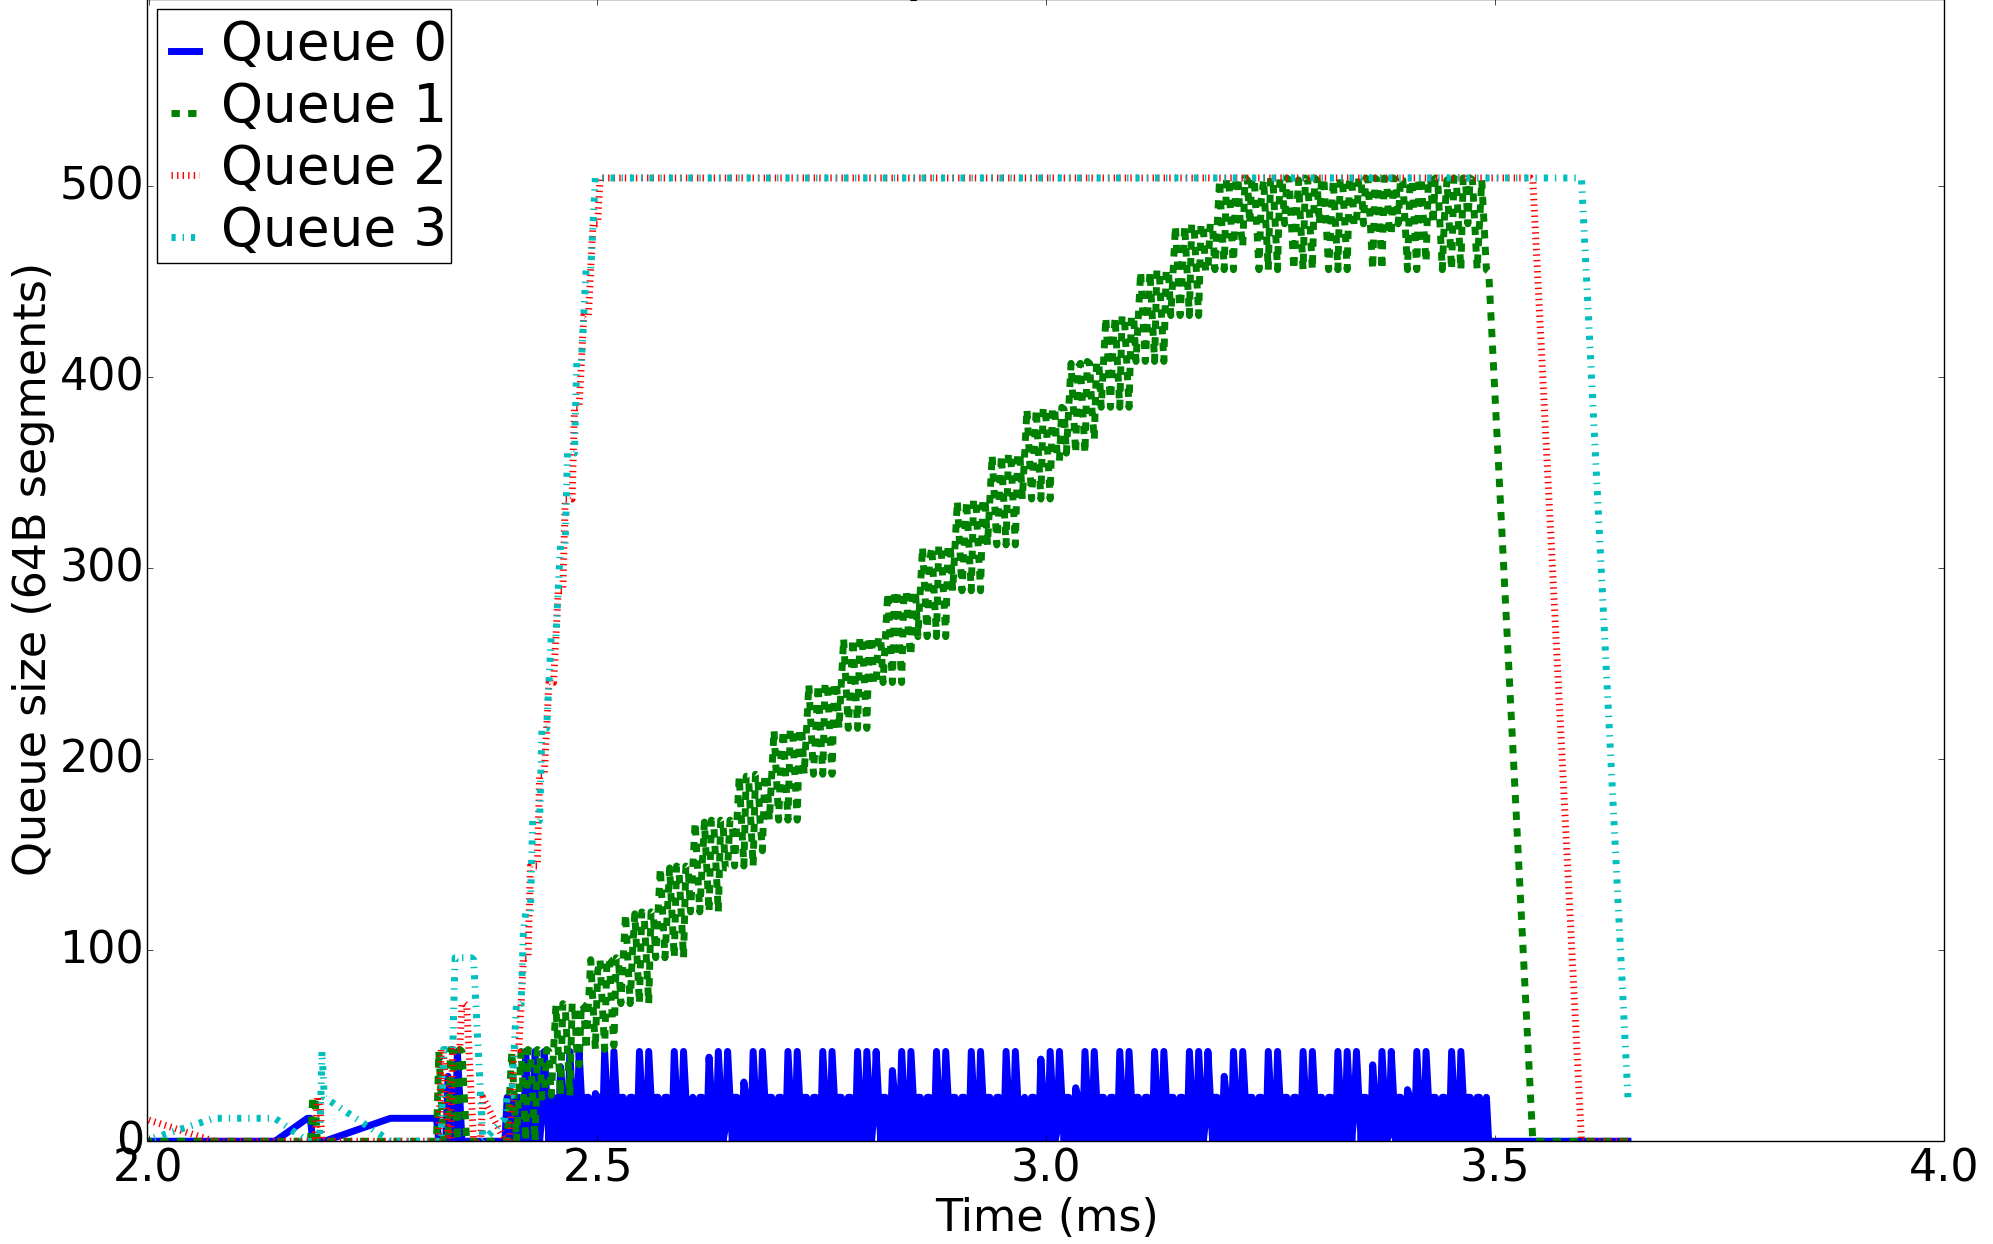
\includegraphics[width=1\linewidth]{figures/eval/strict_queues}
\caption{Queue sizes during strict priority scheduling experiment using our PIFO implementation. Queue 0 is the highest priority queue, followed by 1, 2, then 3.}
\label{fig:strict_queues}
\end{figure}
\
%\begin{figure}[!ht]
%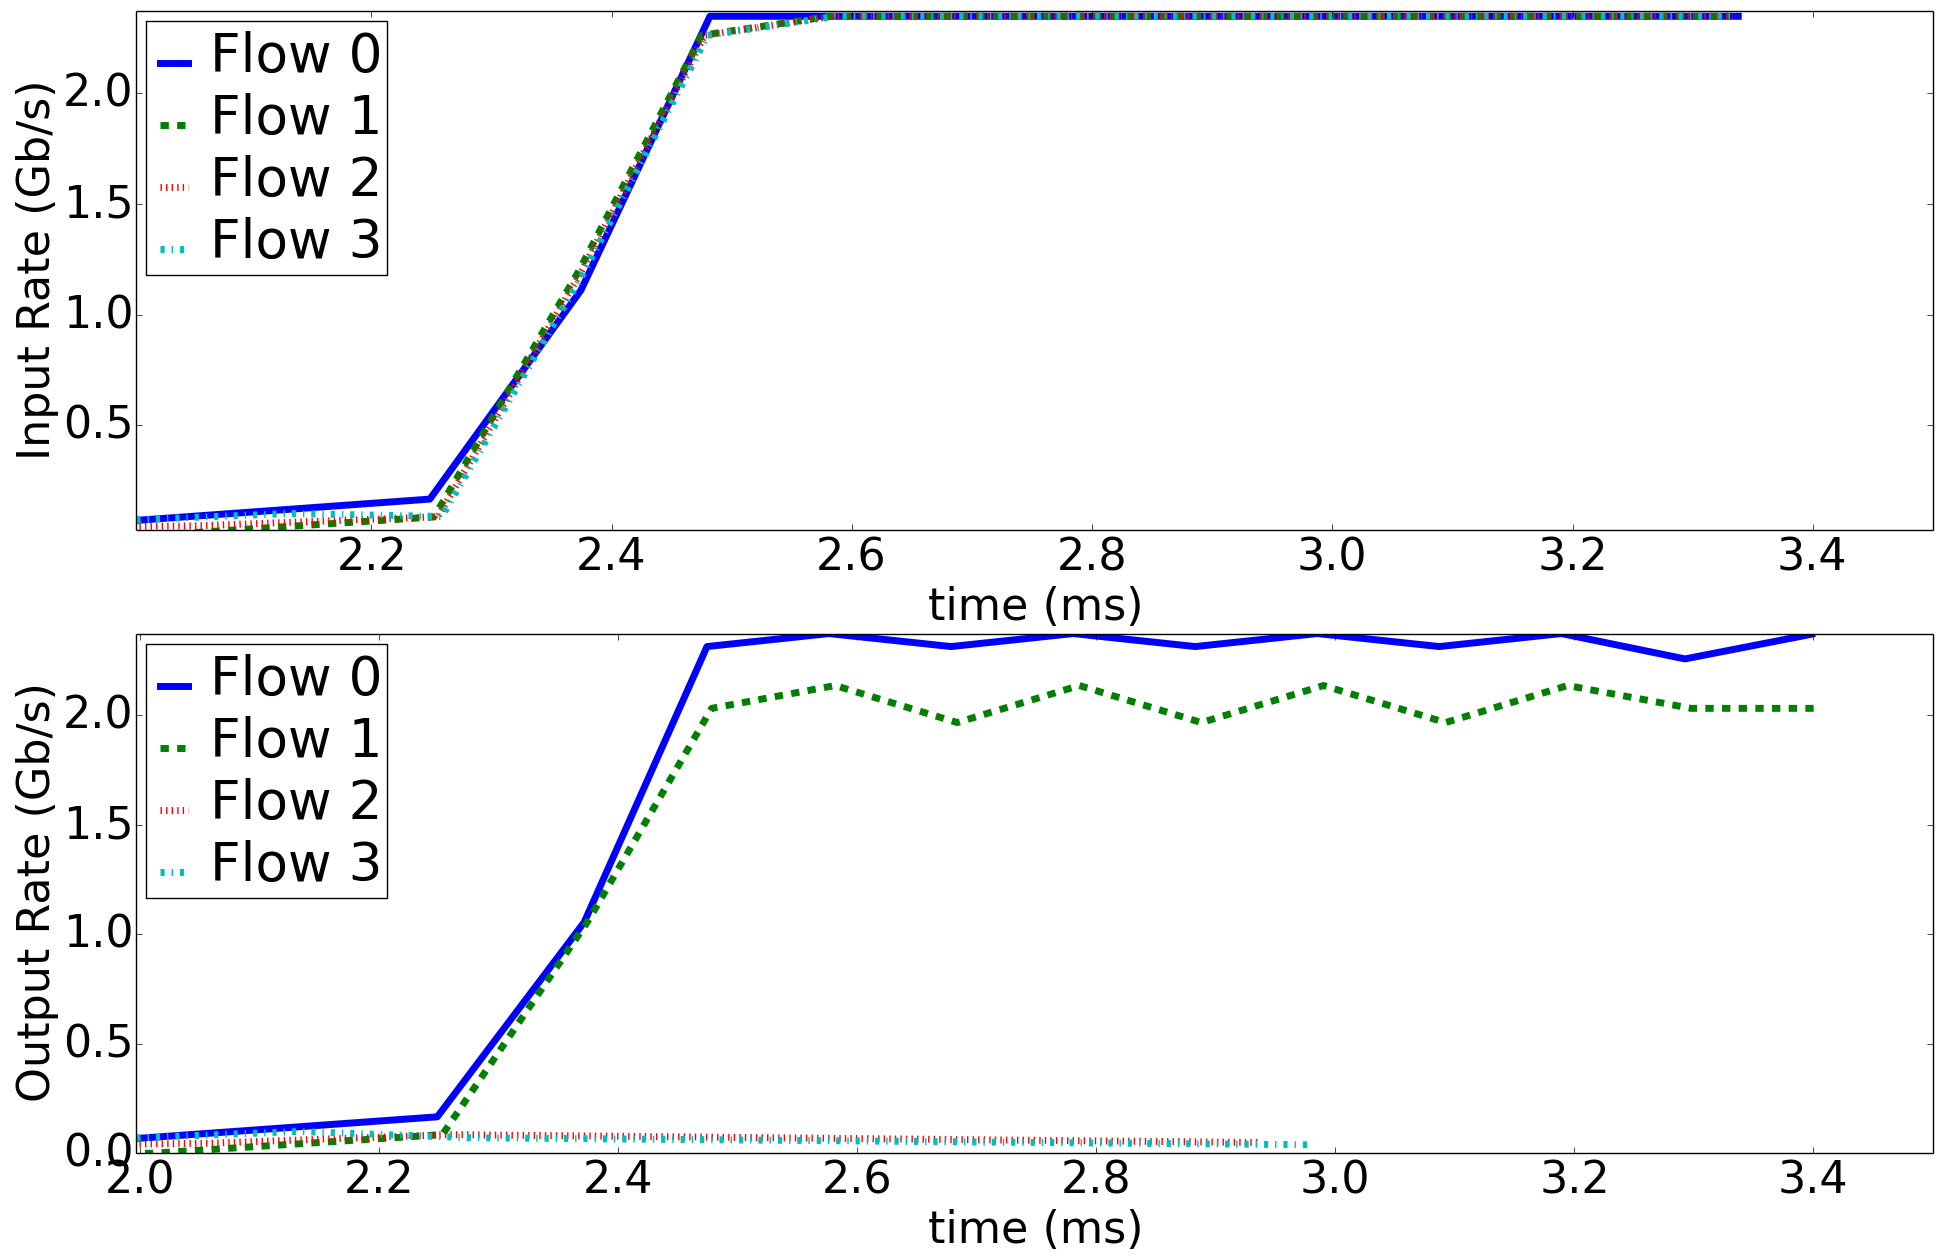
\includegraphics[width=1\linewidth]{figures/eval/strict_rates}
%\caption{Measured input and output flow rates for strict priority scheduling demonstration on the NetFPGA prototype.}
%\label{fig:strict_rates}
%\end{figure}

%\subsection{Round Robin}\label{sec:round-robin}

%\todo[inline]{If needed: remove this section and only show WRR to make room for SRPT discussion.}

%Round robin scheduling is the process of serving a single packet from each queue in an alternating fashion. In order to approximate round robin scheduling using our programmable traffic manager, we changed the rank computation to assign each packet a rank that is equal to the rank of the previous packet in the corresponding flow plus the number of active flows. Figure \ref{fig:rr_rates} shows the measured input and output flow rates for the same four flow workload that was described previously. Since all packets are the same size, we would expect round robin scheduling to evenly share the egress bandwidth between all flows; that is, each flow should receive 1.125 Gb/s. Figure \ref{fig:rr_rates} suggests that the traffic manager is indeed working as expected.

%\begin{figure}[!ht]
%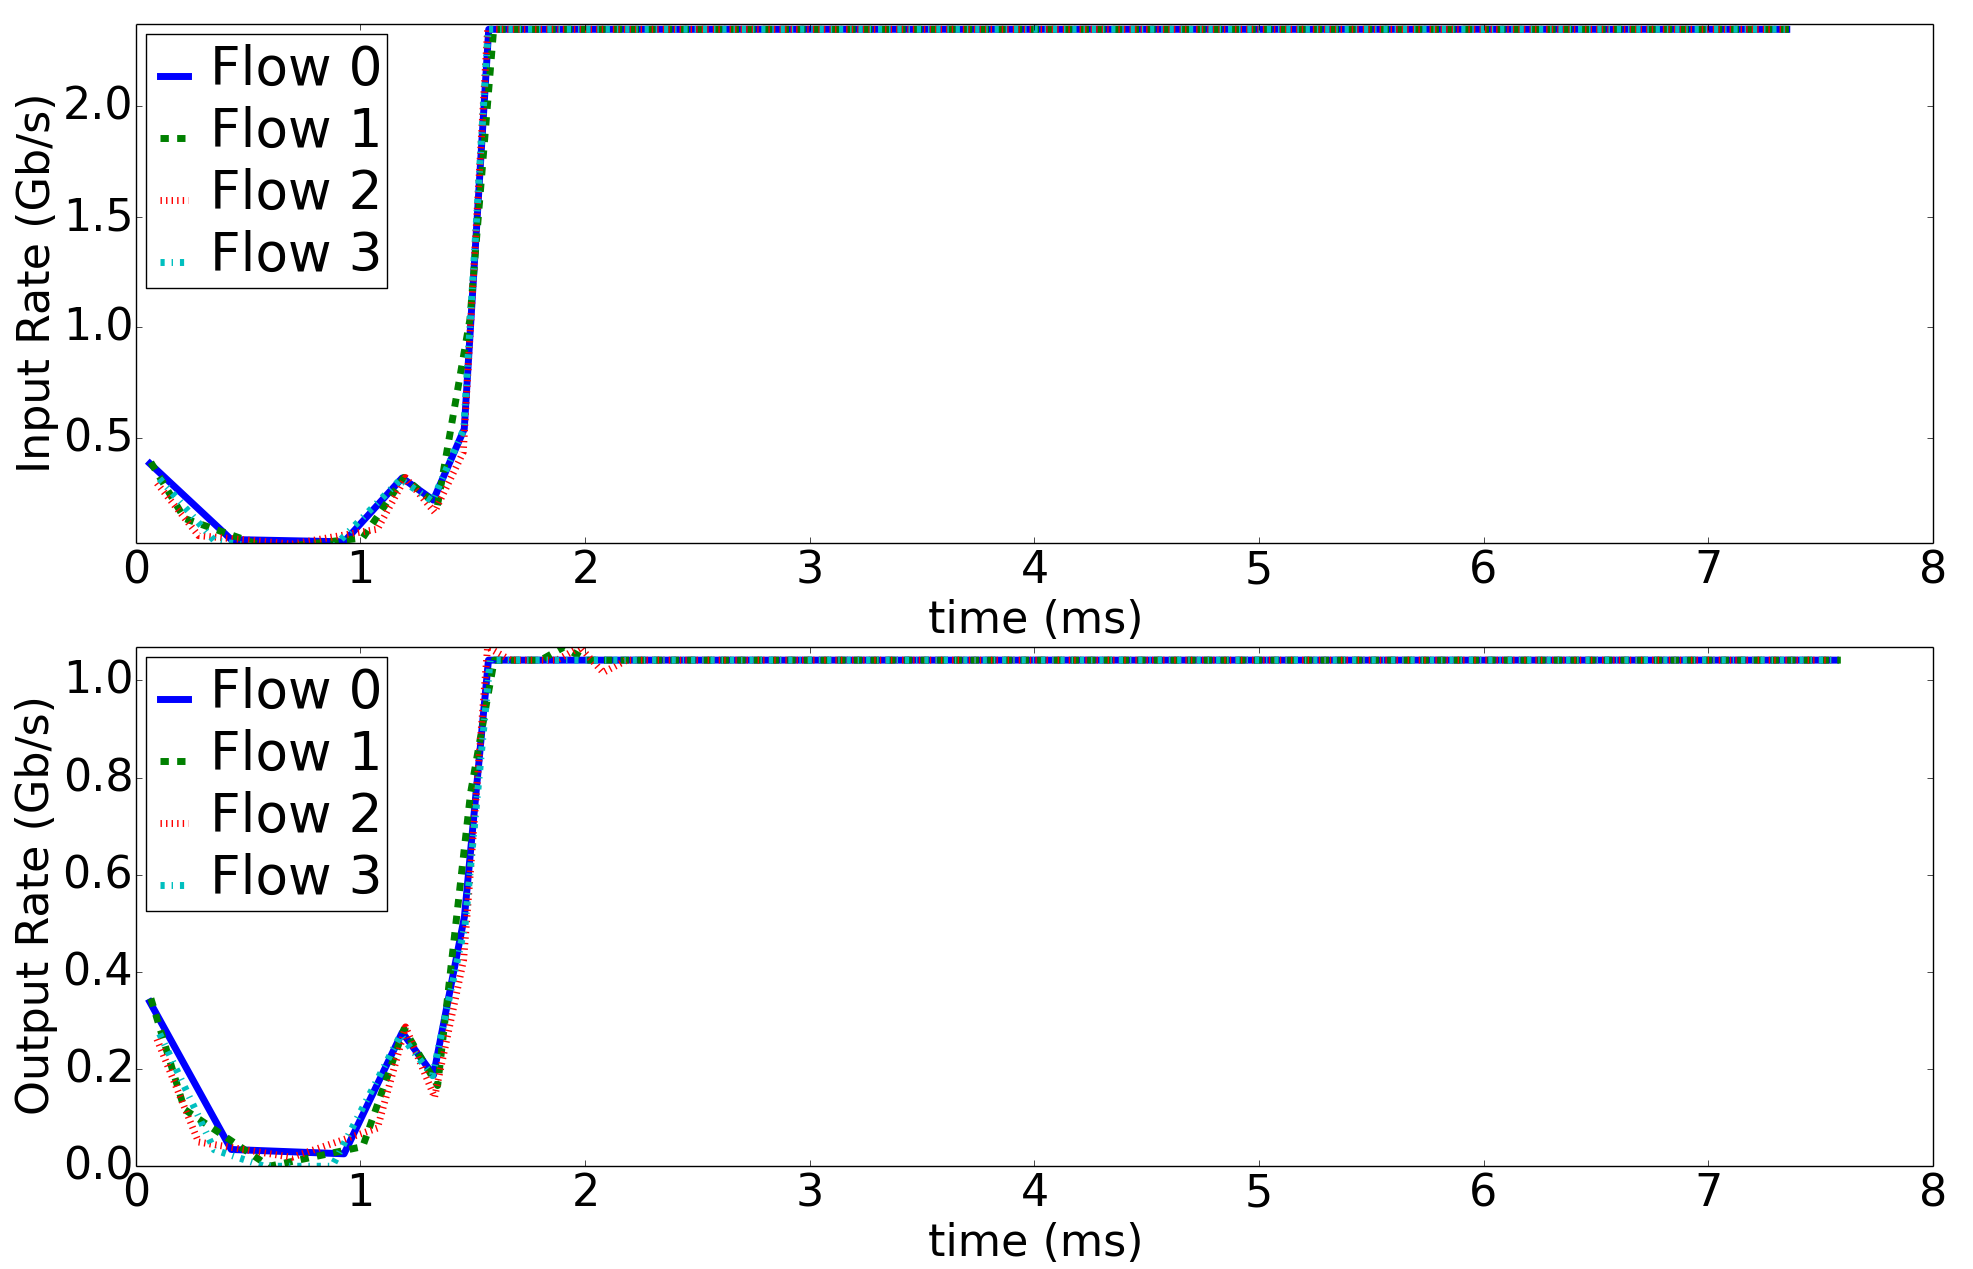
\includegraphics[width=1\linewidth]{figures/eval/rr_rates}
%\caption{Round robin scheduling using our PIFO implementation. All flows are sending 1500B packets.}
%\label{fig:rr_rates}
%\end{figure}

\subsection{Weighted Round Robin}\label{sec:wrr-demo}

Round robin scheduling is the process of serving a single packet from each queue in an alternating fashion.  Weighted round robin scheduling assigns weights to each queue to control its service rate relative to the other queues. In our implementation,  the scheduler dequeues multiple packets from a particular queue according to its weight. We performed an experiment where packet ranks are configured to assign to flow 0 a weight that is twice that of the other three flows. Figure \ref{fig:wrr_rates} shows that this weight factor allows flow 0 to obtain twice as much bandwidth on the egress link relative to the other flows.

\begin{figure}[!ht]
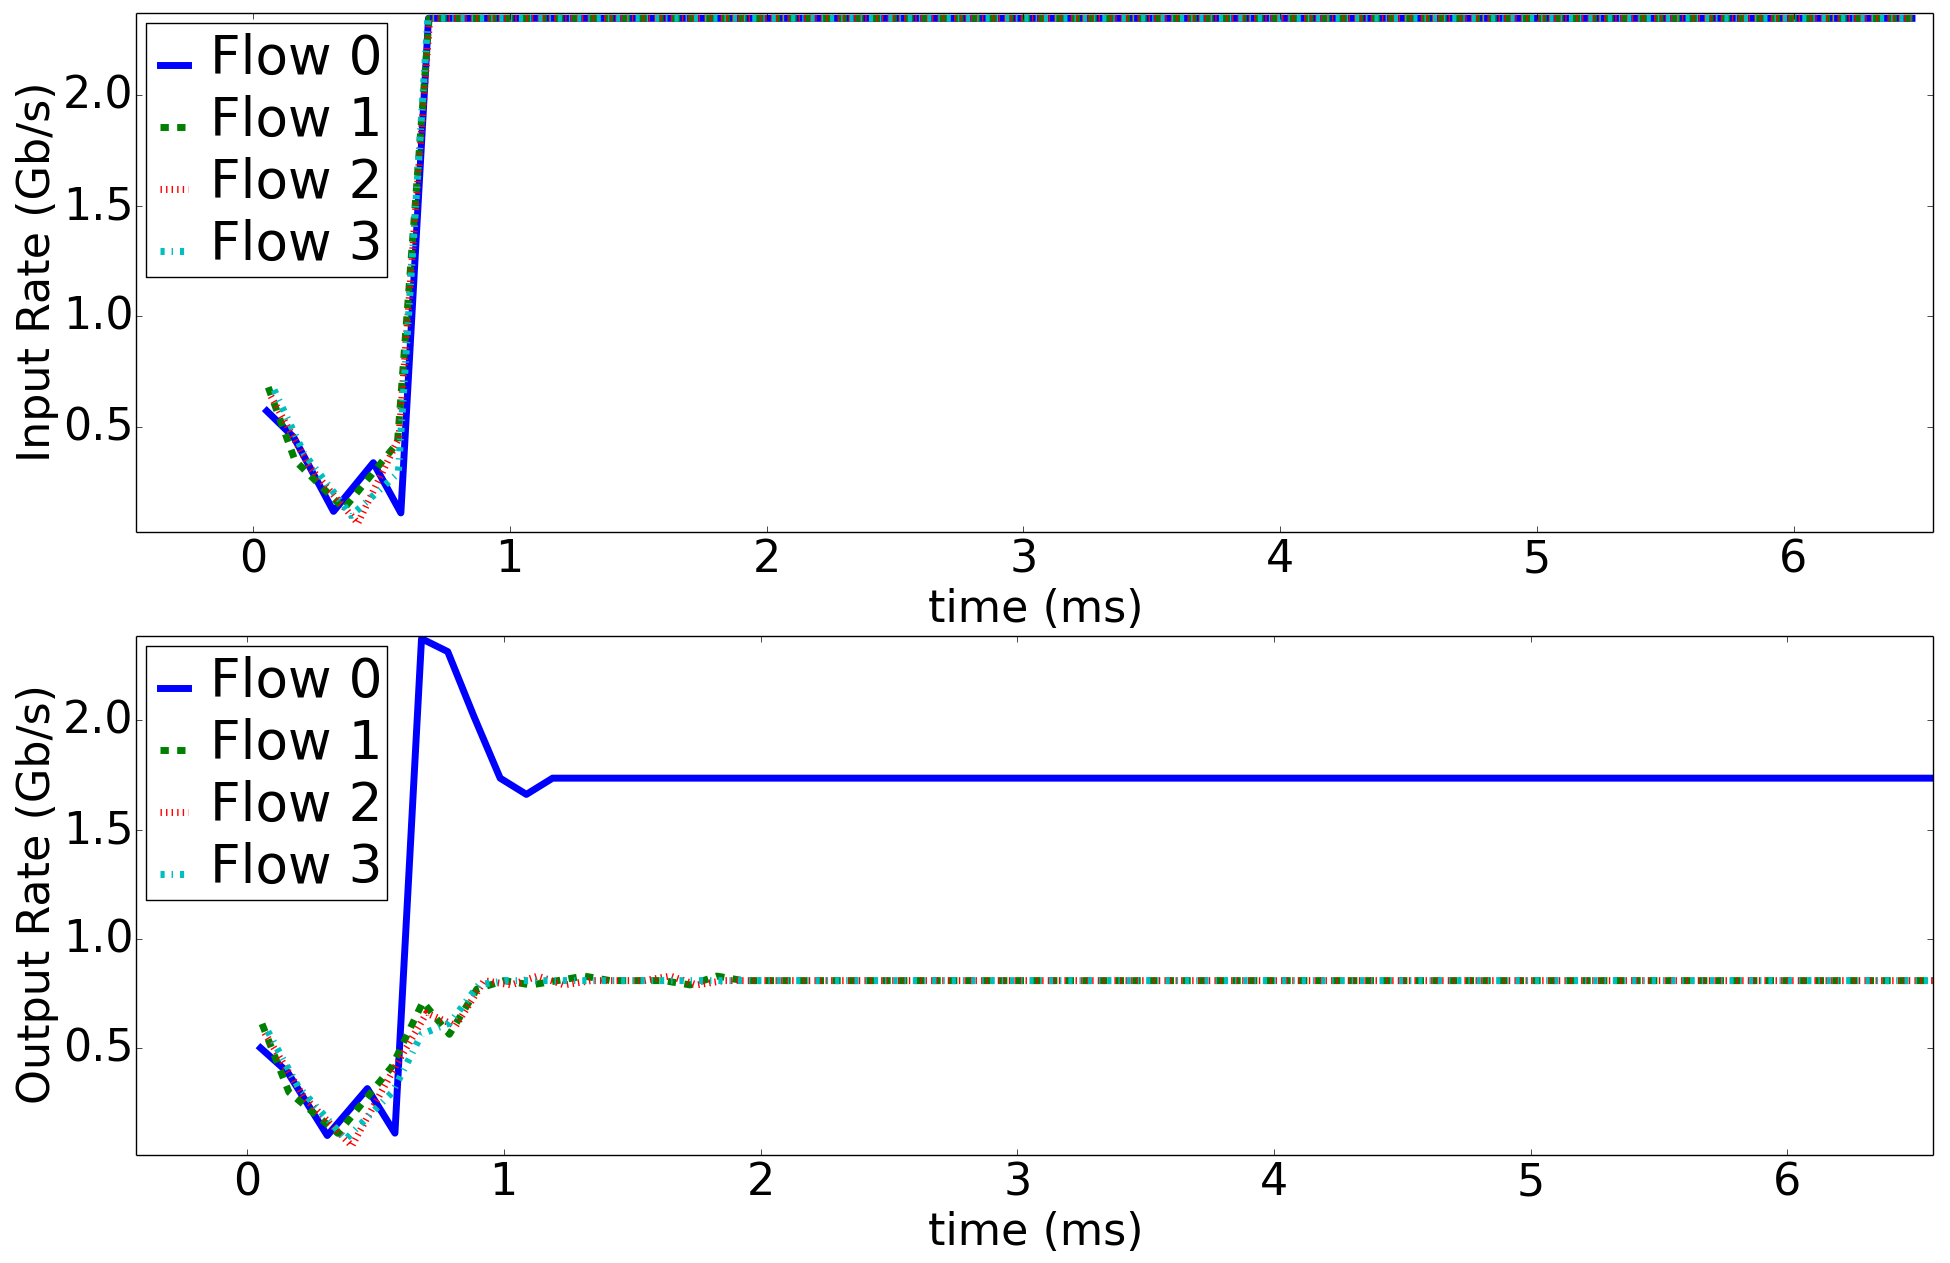
\includegraphics[width=1\linewidth]{figures/eval/wrr_rates}
\caption{Measured input and output flow rates for the weighted round robin scheduling demonstration on the NetFPGA prototype. All flows are sending 1500B packets. Flow 0 is weighted twice as much as the other flows.}
\label{fig:wrr_rates}
\end{figure}

% SRPT Evaluation
\subsection{Shortest Remaining Processing Time (SRPT)}

Shortest Remaining Processing Time (SRPT) is a scheduling algorithm that services first the flow with the least amount of data left to transmit. It is a preemptive version of the shortest flow first algorithm. If a flow arrives that is smaller than the currently active flow, the current flow is preempted and the new smaller flow is serviced. The main benefit of SRPT is that it minimizes the latency experienced by short flows. In the remainder of this section, we describe how we can define the rank computation and queue classification logic to program our traffic manager so that it implements SRPT. We then evaluate our implementation by comparing average small flow completion times for TCP flows that use SRPT versus First-Come-First-Serve (FCFS) scheduling.

\paragraph{Rank Computation}
The PIFO rank computation that is required to implement SRPT is straightforward; the rank is simply assigned to be the remaining flow size. This can either be computed by the switch, or marked in each packet by the source end host. We want the traffic manager to schedule traditional TCP flows, which do not indicate remaining flow size in each packet. TCP flows do, however, use a sequence number which can be used as an indicator of the number of bytes transfered so far. We also commandeer the IP TOS field to serve as an indicator of flow size. It then becomes straightforward to write a simple P4 program that stores the initial sequence number of each flow, and computes the remaining size of the corresponding flow for each packet.

\paragraph{Queue Classification}
The first thing to decide is how to split the buffer space into queues. If you recall from Section \ref{sec:pkt-buf}, our traffic manager implements the tail drop policy. This means that if we use a single queue then it would be possible for a small flow to arrive with no space available in the buffer and subsequently have its packets dropped. An alternative would be to allocate one queue for each flow in order to guarantee that lower priority flows do not consume the buffer space of higher priority flows. However, this approach provides very poor resource sharing and is thus highly impractical. For our SRPT implementation, we decided to partition the buffer space into three queues, one each for long, medium, and short processing times. This approach provides a balanced trade-off between resource sharing and packet priority isolation. Our implementation performs the queue classification logic by performing a ternary match on the computed rank value. This allows a network operator to adjust the queue classification boundaries at runtime by adjusting the table entries.

\paragraph{SRPT Evaluation}
In order to evaluate our SRPT implementation, we compare average small flow completion times (FCT) for TCP with SRPT scheduling and TCP with FCFS scheduling, both of which use a 130KB buffer at the egress link. Figure \ref {fig:srpt_setup} shows the topology that we used for these evaluations. The workload consists of 10 flows: one 45MB flow, one 29MB flow, and eight 1MB flows. These flows are generated using iperf3 and are distributed amongst the two source nodes as shown in Figure \ref{fig:srpt_setup}. Figure \ref{fig:srpt_ranks} shows the SRPT rank values computed for each packet of every flow during one of the experiments. You can clearly see that the implementation is working correctly because Flow 1 (the large flow) is suspended once Flow 2 (a smaller flow) is started at time 40 ms. Furthermore, both Flows 1 and 2 are briefly suspended when any one of the small 1MB flows arrives. Table \ref{tab:fct} shows the average flow completion time of the eight 1MB flows across six runs for both SRPT and FCFS scheduling. We see that by using our SRPT implementation, we can reduce the average FCT of small flows by over 50\%.

\begin{table}[tbp]
\centering
\caption{Comparison of average small flow completion time for TCP with SRPT scheduling and TCP with FCFS scheduling.}
\label{tab:fct}
\begin{tabular}{c|c}
\textbf{Algorithm} & \textbf{Average FCT of small flows (ms)} \\ \hline
TCP with SRPT      & $2.90 \pm 1.63$                          \\ \hline
TCP with FCFS      & $6.00 \pm 3.78$                         
\end{tabular}
\end{table}

\begin{figure}[!ht]
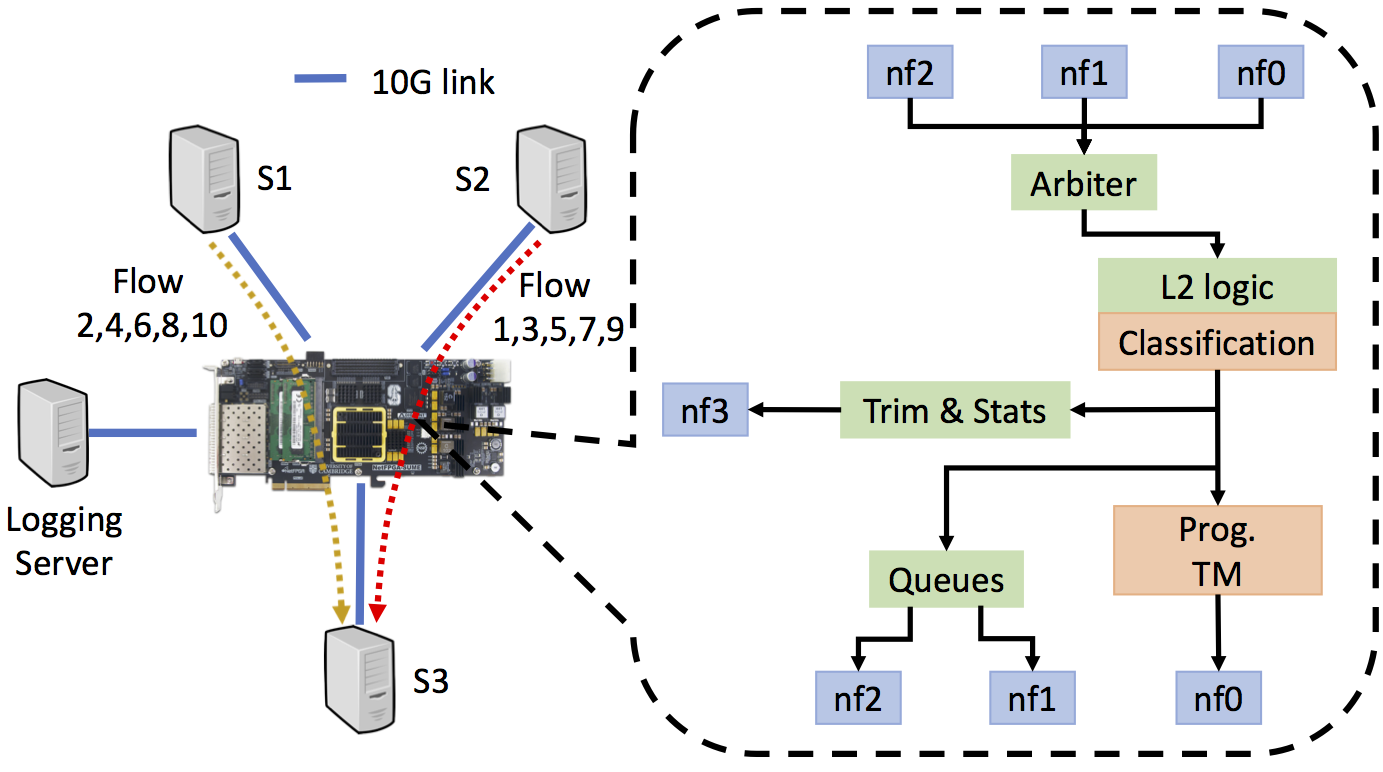
\includegraphics[width=1\linewidth]{figures/design/SRPT-setup}
\caption{The topology, workload, and NetFPGA architecture used for the SRPT evaluations.}
\label{fig:srpt_setup}
\end{figure}

\begin{figure}[!ht]
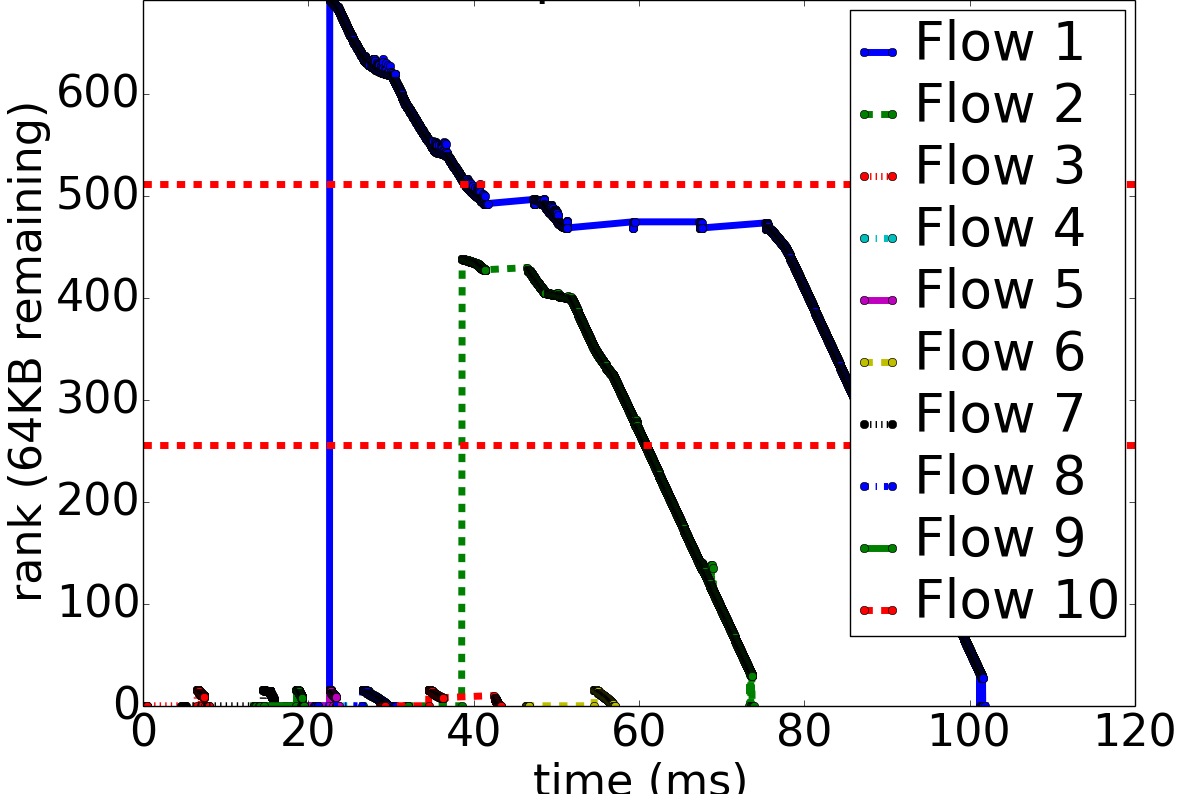
\includegraphics[width=1\linewidth]{figures/eval/srpt_ranks}
\caption{Rank values computed by the switch for each packet during an SRPT experiment. The horizontal dashed red lines indicate the queue classification boundaries. Packets at the top, middle, and bottom are inserted into queues 2, 1, and 0, respectively.}
\label{fig:srpt_ranks}
\end{figure}

\subsection{Utilization Summary}
We compiled our PIFO onto a Virtex-7 FPGA in order to calculate the resource utilization and verify that the design meets all timing constraints. Table \ref{tab:utilization} provides a summary of the FPGA resource utilization for a single PIFO.

\begin{table}[tbp]
\centering
\caption{Virtex-7 resource utilization for a single PIFO that uses 12 parallel priority queues and has a total capacity of 2K packet descriptors.}
\label{tab:utilization}
\begin{tabular}{c|c}
\textbf{Resource} & \textbf{Utilization} \\ \hline
LUTs                                    &  61584                                         \\ \hline
FFs                                     &  55593                                         \\ \hline
32Kbit BRAM Tiles                       &  48
\end{tabular}
\end{table}


